\chapterimage{out.png}
\chapter{Processing}
O Processing é uma linguagem/ferramenta de programação baseada na linguagem de programação Java.
A ideia por detrás da génese do Processing era a criação de uma linguagem para programação de efeitos visuais que
fosse mais fácil de utilizar do que as existentes. Basicamente, o Processing simplifica a programação ao esconder alguns conceitos e alguma da complexidade da programação em Java, ao mesmo tempo de fornece um ambiente de ensino da programação orientado para artistas digitais.

Este capítulo procura enquadrar a utilização do Processing mostrando alguns exemplos de projectos, descreve o ambiente de desenvolvimento da ferramenta e aborda alguns conceitos básicos associados.

\section{O Que É?, Para Que Serve?}
A linguagem Processing tem sido utilizada predominantemente para aplicações artistícas. O Processing pode ser utilizado para instalações, \emph{web art}, \emph{video art}, etc. De seguida apresentam-se alguns projectos em que o Processing foi utilizado.

\begin{description}
\item[Nulltidão] Projecto desenvolvido por João Cordeiro no âmbito da cadeira de Programação Multimédia, em 2006. 
Este projecto consiste numa instalação vídeo que joga com os conceitos de multidão e individualidade. 
A instalação consiste num \emph{video-wall} que exibe um vídeo obtido em tempo-real a partir de uma \emph{web cam}. O vídeo
é manipulado de forma a mostrar apenas algumas regiões da imagem da \emph{web cam} sobrepostas a uma imagem inicial. A imagem inicial é uma \emph{frame} da \emph{web cam} tirada durante a montagem da instalação, de forma a não conter pessoas na imagem. O número de regiões do vídeo depende do número de pessoas a observar a instalação
A instalação usa a informação sobre a quantidade de dispositivos Bluetooth (telemóveis) perto da instalação como estimativa do número de pessoas a observar a instalação. 
\begin{center}
	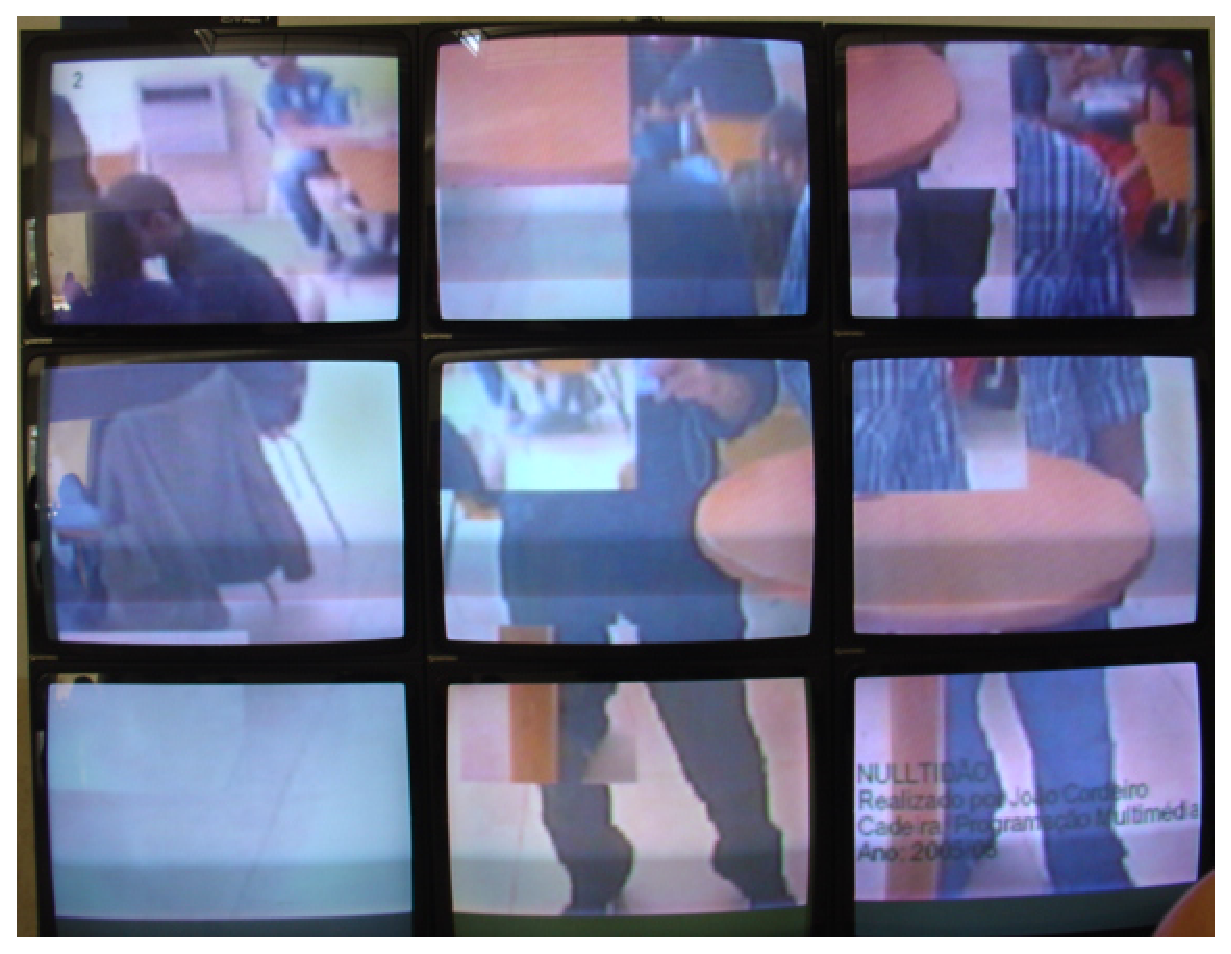
\includegraphics[width=8cm]{images//nulltidao}
\end{center}

\item[Shadow Monsters] \emph{Shadow Monsters} (\url{http://www.worthersoriginal.com/viki/#page=shadowmonsters}) é uma instalação interactiva que permite aos utilizadores projectarem sombras com as mãos. As sombras são modificadas de forma a se transformarem em monstros. 
\begin{center}
	
\includegraphics{images/shadowmonsters.eps}
\end{center}

\item[Nike 'One'] O anúncio realizado pela Motion Theory para a Nike (\url{http://www.motiontheory.com/work/nike_one}) foi programado parcialmente em Processing. O programa utilizado pode ser visto separadamente em \url{http://dev.motiontheory.com/nikegolf/}.
\begin{center}
	
\includegraphics{images/nikeone.eps}
\end{center}

\item[The Dumpster]
O \emph{Dumpster} (\url{http://artport.whitney.org/commissions/thedumpster/}) é uma ``visualização \emph{online} que tenta 
mostrar uma fatia da vida romântica dos adolescentes Americanos. A aplicação usa \emph{posts} reais extraídos de milhões
de blogs e gera uma visualização que permite navegar entre as secções em que uma pessoa ``acabou'' com outra.''.
O projecto foi desenvolvido por Golan Levin, entre outros.
\begin{center}
	
\includegraphics{images/wefeelfine.eps}
\end{center}

\end{description}

\section{Ambiente de Desenvolvimento}
O ambiente de desenvolvimento (\emph{Integrated Development Environment} -- IDE) do Processing é um pequeno editor que permite escrever e executar os programas. 
A Figura~\ref{fig:ide} mostra a janela do IDE. 
\begin{figure}[!hbp]
	\centering
		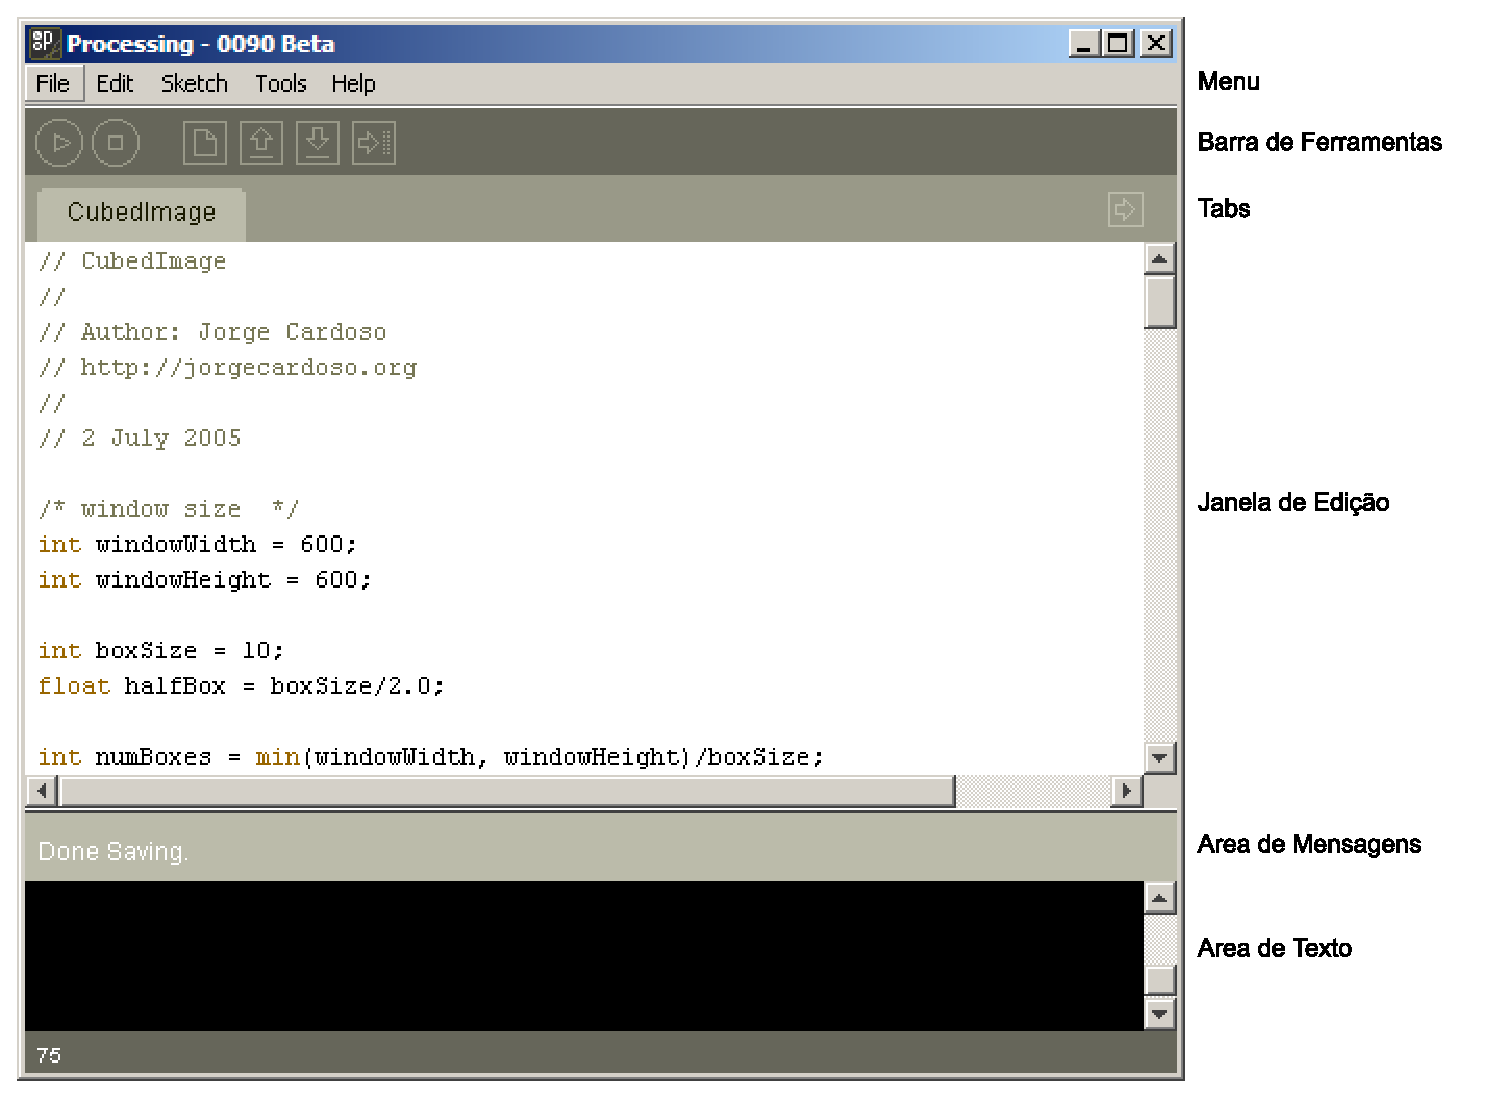
\includegraphics[width=.9\textwidth]{images/ide.eps}
	\caption{IDE do Processing}
	\label{fig:ide}
\end{figure}

A janela do editor está organizada, de cima para baixo, nos seguintes componentes:
\begin{description}
\item[Menu] ... descritos mais à frente.
\item[Barra de Ferramentas] Fornece um acesso rápido às funções Executar, Parar, Criar Novo Sketch, Abrir Sketch, Gravar Sketch e Exportar.
\item[\emph{Tabs}] Cada \emph{Tab} representa um \emph{sketch} aberto.
\item[Janela de Edição] A janela onde escrevemos o código do programa. A janela de edição possui \emph{sintax highlighting}.
\item[Área de Mensagens] Nesta área aparecem algumas mensagens de \emph{status} e os erros de compilação do programa.
\item[Área de Texto] Nesta área é mostrada a saída normal do programa bem como os possíveis erros que ocorram durante a execução.
\end{description}

\subsection{Menus}
Os menus do IDE são os seguintes:
\paragraph{File}
\begin{itemize} 
\item[New] Cria um novo \emph{sketch}.
\item[Sketchbook] Permite abrir um \emph{sketch} localizado no computador, ou um exemplo.
\item[Save] Grava o \emph{sketch} corrente.
\item[Save as...] Grava o \emph{sketch} corrente com um nome diferente.
\item[Export] Exporta o programa como uma \emph{applet} Java e correpondente ficheiro HTML.
\item[Export Application] Exporta o programa como uma aplicação Java para os sistemas Windows, Mac OS X e Linux. 
\item[Page Setup] (Não implementado ainda).
\item[Print] (Não implementado ainda).
\item[Preferences] Abre a janela de configuração do Processing.
\item[Quit] Termina o IDE e fecha todas as janelas.
\end{itemize}

\paragraph{Edit}
\begin{itemize}
\item[Undo] Desfaz o último commando aplicado.
\item[Redo] Desfaz o Undo.
\item[Cut] Remove e copia para o \emph{clipboard} o texto seleccionado.
\item[Copy] Copia para o \emph{clipboard} o texto seleccionado.
\item[Paste] Insere o conteúdo do \emph{clipboard} na posição do cursor.
\item[Select All] Selecciona todo o texto da janela de edição.
\item[Find] Procura uma ocorrência de uma palavra no texto e dá a opção de o substituir por outra palavra.
\item[Find Next] Procura a próxima ocorrência de uma palavra no texto.
\end{itemize}

\paragraph{Sketch}
\begin{itemize}
\item[Run] Executa o código. Este comando faz automaticamente a compilação do programa, abre a janela do programa e executa-o.
\item[Present] Executa o programa em \emph{fullscreen}.
\item[Stop] Se o programa estiver a executar, este comando termina-o.
\item[Add File] Permite adicionar um ficheiro de imagem ou outro tipo de dados à pasta de dados do projecto.
\item[Import Library] Adiciona as instruções de \emph{import} das bibliotecas ao programa corrente.
\item[Show Sketch Folder] Abre a pasta do projecto.
\end{itemize}

\paragraph{Tools}
\begin{itemize}
\item[Auto Format] Tenta formatar o código de forma a torná-lo mais legível.
\item[Create Font] Converte fontes no formato de fontes do Processing.
\item[Archive Sketch] Cria um ficheiro zip com o conteúdo do projecto.
\end{itemize}

\paragraph{Help}
\begin{itemize}
\item[Environment] Abre a página que descreve o ambiente de desenvolvimento do Processing.
\item[Reference] Abre  a página que contém a referência das funções do Processing.
\item[Find in Reference] Procura na referência, a palavra seleccionada no editor de texto.
\item[Visit Processing.org] Abre a página do Processing.org.
\item[About Processing] Painel de informação sobre o software.
\end{itemize}

\section{Obter o Processing}
O Processing pode ser descarregado a partir do site \url{processing.org}. Na secção \emph{download} existe a opção de descarregar 4 versões: duas para Windows (com ou sem Java -- devem descarregar a versão com Java), uma para Mac OS X e uma para Linux.



\section{Coordenadas}
O Processing utiliza um sistema de coordenadas cartesiano com a origem das coordenadas localizada no canto superior esquerdo do ecrã. O eixo dos XX é positivo para a direita e o eixo dos YY é positivo para baixo. No caso de estarmos a trabalhar em 3D, o eixo dos ZZ é positivo na direcção do utilizador.

A Figura~\ref{fig:coordinates} exemplifica o sistema de coordenadas.
\begin{figure}[htbp]
	\centering
		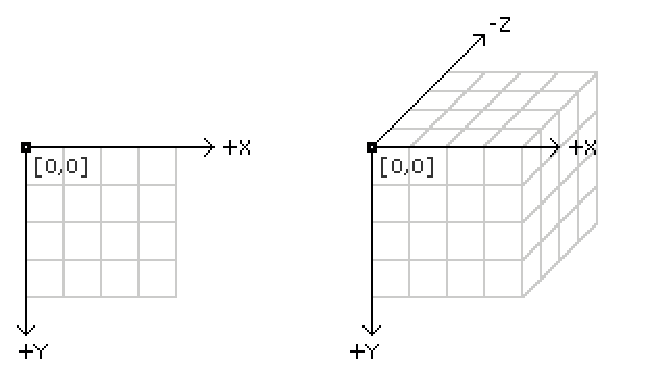
\includegraphics[width=10cm]{images/coordinates.eps}
	\caption{Sistema de coordenadas em Processing}
	\label{fig:coordinates}
\end{figure} 

\section{Compilar, Executar e Publicar}
Os programas em Processing precisam de ser compilados antes de serem executados. No entanto, no ambiente Processing, estes dois passos estão intimamente ligados: quando pressionamos no botão de executar, o nosso programa é automaticamente compilado e só depois executado.

A maior parte dos programas Processing são apresentados via Web, ou seja, são colocados numa página com uma applet. Para publicarmos o nosso programa, basta-nos aceder ao menu [File->Export]. Automaticamente, o Processing cria uma pasta nova dentro da pasta do nosso projecto com o nome \texttt{applet}. Nesta pasta encontramos cinco ficheiros:
\begin{description}
\item[index.html] A página html principal. Esta página contém o código que inclui a applet. 

\item[loading.gif] Uma imagem utilizada na applet enquanto o nosso programa está a ser carregado.

\item[NomeProjecto.jar] O nosso programa compilado e empacotado num ficheiro jar%
\footnote{Um ficheiro jar é basicamente um ficheiro comprimido (zip) com os ficheiros que compõem o nosso programa.}%
.

\item[NomeProjecto.java] O nosso programa Processing convertido em Java.

\item[NomeProjecto.pde] O nosso código fonte.
\end{description}

Se quisermos colocar o nosso programa online basta-nos copiar esta pasta para um servidor Web.

Uma outra forma de distribuir o nosso programa é através de uma aplicação que execute directamente no nosso computador (ao invés de executar através de um browser Web). Também podemos converter o nosso programa numa aplicação com o ambiente Processing. Para tal temos de aceder ao menu [File->Export Application]. Automaticamente, o Processing cria três pastas: \texttt{application.linux}, \texttt{application.macosx} e \texttt{application.windows}. Estas pastas contém as três versões da nossa aplicação, uma para cada sistema operativo.

\section{Alguns Exemplos}
\lstset{basicstyle=\scriptsize\ttfamily}

A partir desta secção o código utiliza a sintaxe do Processing.

Os exemplos seguintes foram retirados do site do Processing. 
Estes exemplos vêm com o Processing quando se descarrega e podem também ser vistos online na secção de exemplos da página do Processing.

\paragraph{Statements and Comments (Instruções e Comentários)}
\begin{center}

\includegraphics[width=4cm]{images/exemploStatementsComments.eps}
\end{center}
\begin{lstlisting}
// Statements and Comments
// by REAS <http://reas.com>

// Statements are the elements that make up programs.
// The ";" (semi-colon) symbol is used to end statements. 
// It is called the "statement terminator."
// Comments are used for making notes to help people better understand programs. 
// A comment begins with two forward slashes ("//").

// Created 1 September 2002

// The size function is a statement that tells the computer 
// how large to make the window.
// Each function statement has zero or more parameters. 
// Parameters are data passed into the function
// and used as values for specifying what the computer will do.
size(200, 200);

// The background function is a statement that tells the computer
// which color to make the background of the window 
background(102);
\end{lstlisting}

\paragraph{Width and Height (Largura e Altura)}
\begin{center}

\includegraphics[width=4cm]{images/exemploWidthHeight.eps}
\end{center}
\begin{lstlisting}
// Width and Height
// by REAS <http://reas.com>

// The 'width' and 'height' variables contain the width and height 
// of the display window as defined in the size() function.

// Created 27 October 2002

size(200, 200);
background(127);
noStroke();
for(int i=0; i<height; i+=20) {
  fill(0);
  rect(0, i, width, 10);
  fill(255);
  rect(i, 0, 10, height);
}
\end{lstlisting}



\section[Modos de Programação]{Modos de Programação\protect\footnote{Traduzido e adaptado de \cite{Processing.orgProcessingEnvironmentVisitadoJaneiro2007}.}}
O Processing permite-nos programar em três níveis diferentes de complexidade: Modo Básico,
Modo Contínuo e Modo Java.
Deve-se começar pelo modo Básico para aprender a trabalhar com coordenadas, variáveis e ciclos antes
de passar para o modo Contínuo e modo Java.

\subsection{Modo Básico}
Neste modo apenas podemos programar imagens estáticas. Este modo é utilizado principalmente para aprender os fundamentos da programação. 
O exemplo seguinte desenha um rectângulo amarelo no ecrã%
\footnote{Todas as instruções neste exemplo são chamadas a métodos do Processing. Um método, ou função, é uma instrução básica do Processing, ou um agrupamento
de instruções básicas que se comporta como uma instrução básica. Os valores entre parentesis são os argumentos do método, i.e., valores que alteram a forma como o método se comporta. Os métodos são explicados no Capítulo~\ref{cap:metodos}.}
:
\begin{lstlisting}
size(200, 200);         // definir o tamanho da janela
background(255);        // colocar o fundo a branco
noStroke();             // indicar que as formas não têm border
fill(255, 204, 0);      // definir a cor de preenchimento - amarelo
rect(30, 20, 50, 50);   // desenhar um rectângulo (50x50) 
                        // na posição (30, 20)
\end{lstlisting}
Neste modo as instruções são interpretadas uma a uma e o programa termina quando a última for encontrada.

\subsection{Modo Contínuo}
O modo Contínuo fornece uma estrutura de programação em que é possível desenhar continuamente para o ecrã. Desta forma podemos construir animações. Neste modo é também possível obter \emph{input} do utilizador através do teclado e do rato.

Na sua forma mais básica, um programa neste modo é constituído por dois métodos: \texttt{setup()} e \texttt{draw()}. O método \texttt{setup()} serve para inicializar o programa -- este método executa apenas uma vez. O método \texttt{draw()} permite-nos desenhar para o ecrã -- este método é invocado repetidamente pelo sistema, permitindo-nos construir animações.


O exemplo seguinte desenha três círculos azuis semi-transparentes. Neste caso o método \texttt{draw()} apenas é executado uma vez, porque usamos o método \texttt{noLoop()} dentro do \texttt{setup()} para indicar que não queremos animação.
\begin{lstlisting}
void setup()
{
  size(200, 200);           // janela 200x200
  noStroke();               // não desenha linhas
  background(255);          // fundo branco
  fill(0, 102, 153, 204);   // azul com transparencia
  smooth();                 // desenha as formas mais suavemente

  noLoop();                 // draw vai ser chamado apenas uma vez
}

void draw()
{
    /* desenha três círculos  */
    ellipse(100, 150, 100, 100); 
    ellipse(100, 100, 75, 75);
    ellipse(100, 50, 50, 50);
}
\end{lstlisting}

O exemplo seguinte desenha dois quadrados que acompanham a posição do ponteiro do rato (a posição do ponteiro está guardada nas variáveis \texttt{mouseX} e \texttt{mouseY}). O método \texttt{draw()} é invocado continuamente até o programa ser terminado, permitindo-nos interagir e criar movimento com os quadrados.
\begin{lstlisting}
void setup()
{
    // Janela de 200x200
    size(200, 200);          
  
    // A referência do rectângulo é o seu centro
    rectMode(CENTER);        
    
    // Não desenhamos linhas
    noStroke();              
  
    // Preenchimento de formas com a cor azul semi-transparente  
    fill(0, 102, 153, 204);  
}
void draw()
{
    // fundo azul
    background(255);                           

    // desenhar um quadrado na posição simétrica da do ponteiro do rato
    rect(width-mouseX, height-mouseY, 50, 50); 
  
    // desenhar outro quadrado na posição do ponteiro do rato
    rect(mouseX, mouseY, 50, 50);
}
\end{lstlisting}

\subsection{\emph{Java}}
Este modo de programação do Processing é o mais flexível porque permite-nos ter acesso às bibliotecas completas do Java.




\section{Exercícios}
\begin{enumerate}

\item 
Procurar na Internet outros projectos em que o Processing é utilizado. Descrevê-los.

\item 
Descarregar e instalar o Processing o seu computador.
Executar o Processing e abrir alguns dos exemplos. Compilar, executar e publicar pelo menos 3 exemplos. Colocar os programas online.

\item
Escolher um entre os seguintes exemplos do site do Processing:
\begin{itemize}
\item \label{exe:2_1}
*
Setup and Draw -- \url{http://processing.org/learning/examples/setupdraw.html}

\item
Points and Lines -- \url{http://processing.org/learning/examples/pointslines.html}

\item
Integers and Floats -- \url{http://processing.org/learning/examples/integersfloats.html}

\item
Variables -- \url{http://processing.org/learning/examples/variables.html}

\item
Iteration -- \url{http://processing.org/learning/examples/iteration.html}
\end{itemize}
Explicar o que faz \textbf{cada linha de código} do exemplo escolhido. Uma forma de tentar perceber o que faz cada linha é correr o programa com apenas essa linha e ver o resultado. Colocar a resolução online num ficheiro de texto com o nome do exemplo escolhido.
\end{enumerate}